\documentclass[12pt]{article}
% Preamble
\usepackage[left=2cm,top=1cm,right=2cm,nohead,nofoot]{geometry}
\usepackage[pdftex]{graphicx}

% Header
\title{ECE457 Project 1}
\author{Daniel Burstyn (20206120)}
\date{Oct 14, 2009}

% Body
\begin{document}
\maketitle

\section{Comparison of algorithms for two-point-problem}
Breadth First Search (BFS), Depth First Search (DFS) and A-Star search
algorithms were all run on the two-point-problem with varying results.  In this
case, Manhattan distance was used as the heuristic for A-Star.\\

In the below table, Expored denotes the number of points that were added to the
open queue, whereas Visited is the number of points that have been actually
visited (they were popped off the open queue.)  Visited is the more important
result because it is directly proportional to how fast the program runs.  Length
is the total length of the net generated, and CPU Time is the amount of time
(user and system) it took to run the search.\\

\vspace{1em}

\begin{center}
\begin{tabular}{| c | c | c | c | c |}
\hline
Algorithm & Explored & Visited & Length & CPU Time \\
\hline
\hline
BFS & 2812 & 2733 & 112 & 28ms \\
\hline
DFS & 1699 & 1233 & 682 & 36ms \\
\hline
A-Star & 1245 & 1093 & 112 & 36ms \\
\hline
\end{tabular}
\end{center}

\vspace{1em}

First of all, we see that the time it took to run each search was low, and the
results are most likely too imprecise to compare to eachother.  Needless to say,
since the size of the two-point-problem was small, each algorithm ran quickly.\\

The next thing we notice is that BFS and A-Star both found paths of length 112,
and DFS found one of length 682.  We know that BFS is optimal, and that A-Star
is optimal in this case since Manhattan distance is admissible, which explains
why they reached the same result.  We also know that depth first search can move
all over the place and the path generated is typically quite bad.\\

Although DFS is not a very smart search, and results in a bad path, we know that
it takes very little memory as we can see from the low visited and explored
count.  Since we have a low number of visited nodes, we also know it runs
comparatively fast but this is only due to luck.  Even the memory usage and time
cost are low, since the result is non-optimal this algorithm is not very useful
for the purpose of this assignment.\\

A-Star on the other hand visited the least, explored the least, and came up with
an optimal path.  Since A-Star is an informed search, it can make much better
decisions about what nodes to visit, which leads to the better results.  Since
A-Star is aware of the goal, the heuristic function allows it to visit nodes in
the direction of the goal---we retain the optimality of BFS without having to
visit too many points.\\

\section{Heuristic for n-point-problem}
The n-point problems are significantly more complex than the two-point-problems
which can be solved optimally.  Because of this, we must take a smarter approach
to connecting the net points.\\

To connect n points, each point is added one by one to the net.  Instead of
choosing the next point at random, we can choose the next point to be the one
closest to the already connected net.  To this, my search program will take the
net points and sort them by distance to the middle of the grid.  I choose to
sort them this way because the computation is inexpensive, and also due to the
natural tendency of most paths to cross through the centre of the grid.\\

Once the points are sorted, they must be connected to eachother one by one.  I
tried two different approaches for this.  The first approach was to use A-Star
since we know that A-Star is both fast and low on memory usage.  Of course,
since we don't have a single point as the goal we need to define a new heuristic
for A-Star to use.  For this I decided to use the minimum of all Manhattan
distances between the point and all points already on the path.  This heuristic
gives benefit to points that are closest to any point on the path, and seemed
like it was suitable for this problem.  Unfortunately, due to the multiple
points of the problem, the heuristic is not admissable and will not necessarily
give the optimal solution.\\

The other approach was to use BFS instead of A-Star.  I found from my tests (see
below) that BFS occasionally produced slightly better (fewer wires) results.
This is most likely just luck based on the placement of points.  The way each
algorighm connects is slightly different (see images below), and this may be a factor in the
result.  At the cost of a slightly better solution, BFS takes longer to run and
uses much more memory.\\

\begin{center}
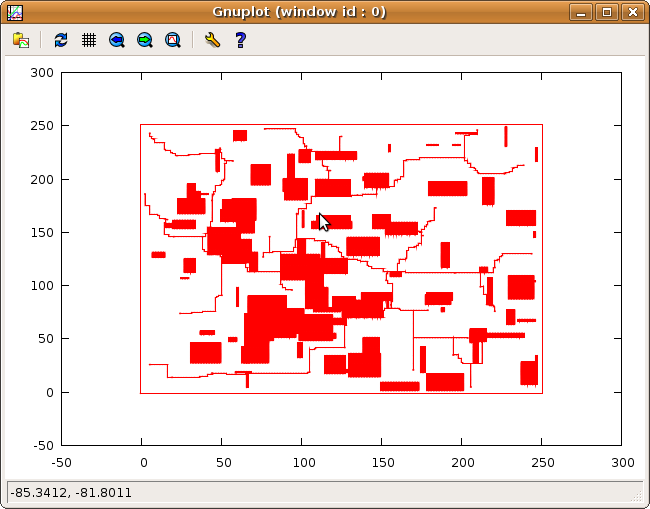
\includegraphics[scale=0.5]{bfs.png}

BFS Solution to n-point-problem-2

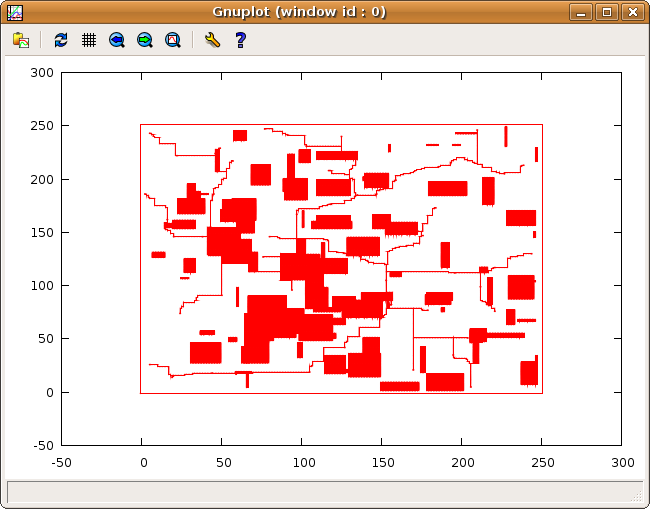
\includegraphics[scale=0.5]{astar.png}

A-Star Solution to n-point-problem-2
\end{center}

\section{Comparison of quality of solutions}
Both of the approaches were tested on all three of the n-point-problems
generating the following results:

\vspace{1em}

\begin{center}
\begin{tabular}{|c|c|c|c|c|c|c|}
\hline
& \multicolumn{3}{|c|}{BFS} &
\multicolumn{3}{|c|}{A-Star} \\
\hline
& Problem 1 & Problem 2 & Problem 3 & Problem 1 & Problem 2 & Problem 3\\
\hline
Visited  & 19296 & 97210  & 347447 & 2112 & 8820  & 25910 \\
Explored & 20229 & 101927 & 362525 & 2981 & 12644 & 37728 \\
Length   & 503   & 1724   & 5222   & 499  & 1737  & 5277 \\
Time     & 0.4s  & 7s     & 75s    & 0.1s & 1s    & 9s   \\
\hline
\end{tabular}
\end{center}

\vspace{1em}

We can see that the number of visited and explored points are much much larger
for BFS than for A-Star.  The results show that BFS explores about 10 times the
number of points that A-Star does, which is of course because A-Star is informed
and can make better decisions about what point to visit next.

These results back up what we learnt from class, and what has
been explained above: that BFS is slower and uses more memory.  The timing
results also show that A-Star is an order of magnitude faster than BFS.\\

The quality of the results, however, is quite close between the two methods.
A-Star is only slightly better for n-point-problem 1, but BFS is better for the
other two cases.\\

In conclusion, by sorting the net points by their distance to the middle of the
grid, we gain a significant improvement in the size of our results.  Using BFS
for connecting the points uses more memory, and is slower, but produces slightly
better results.

\end{document}
